In this section we will present the results of simulations and compare them with previous methods and true optima.

\subsection{Initial condition}
	First we have to check if changing the initial state makes any difference to the output of an algorithm. This is achieved via setting a different seed and repeating algorithms for the same number of iterations. Seeds guarantee us the different ``randomness'' with each seed. It is because the generators are only generating \textit{pseudo-random numbers} which we can control. Both algorithms will have the same seeds and in our case these are $1,2,3,4$. We use default parameters of temperature $\tau=2$ and cooling parameter $t_n=1$.
	\begin{figure}[!htb]
	\centering
	\begin{subfigure}{0.45\textwidth}
		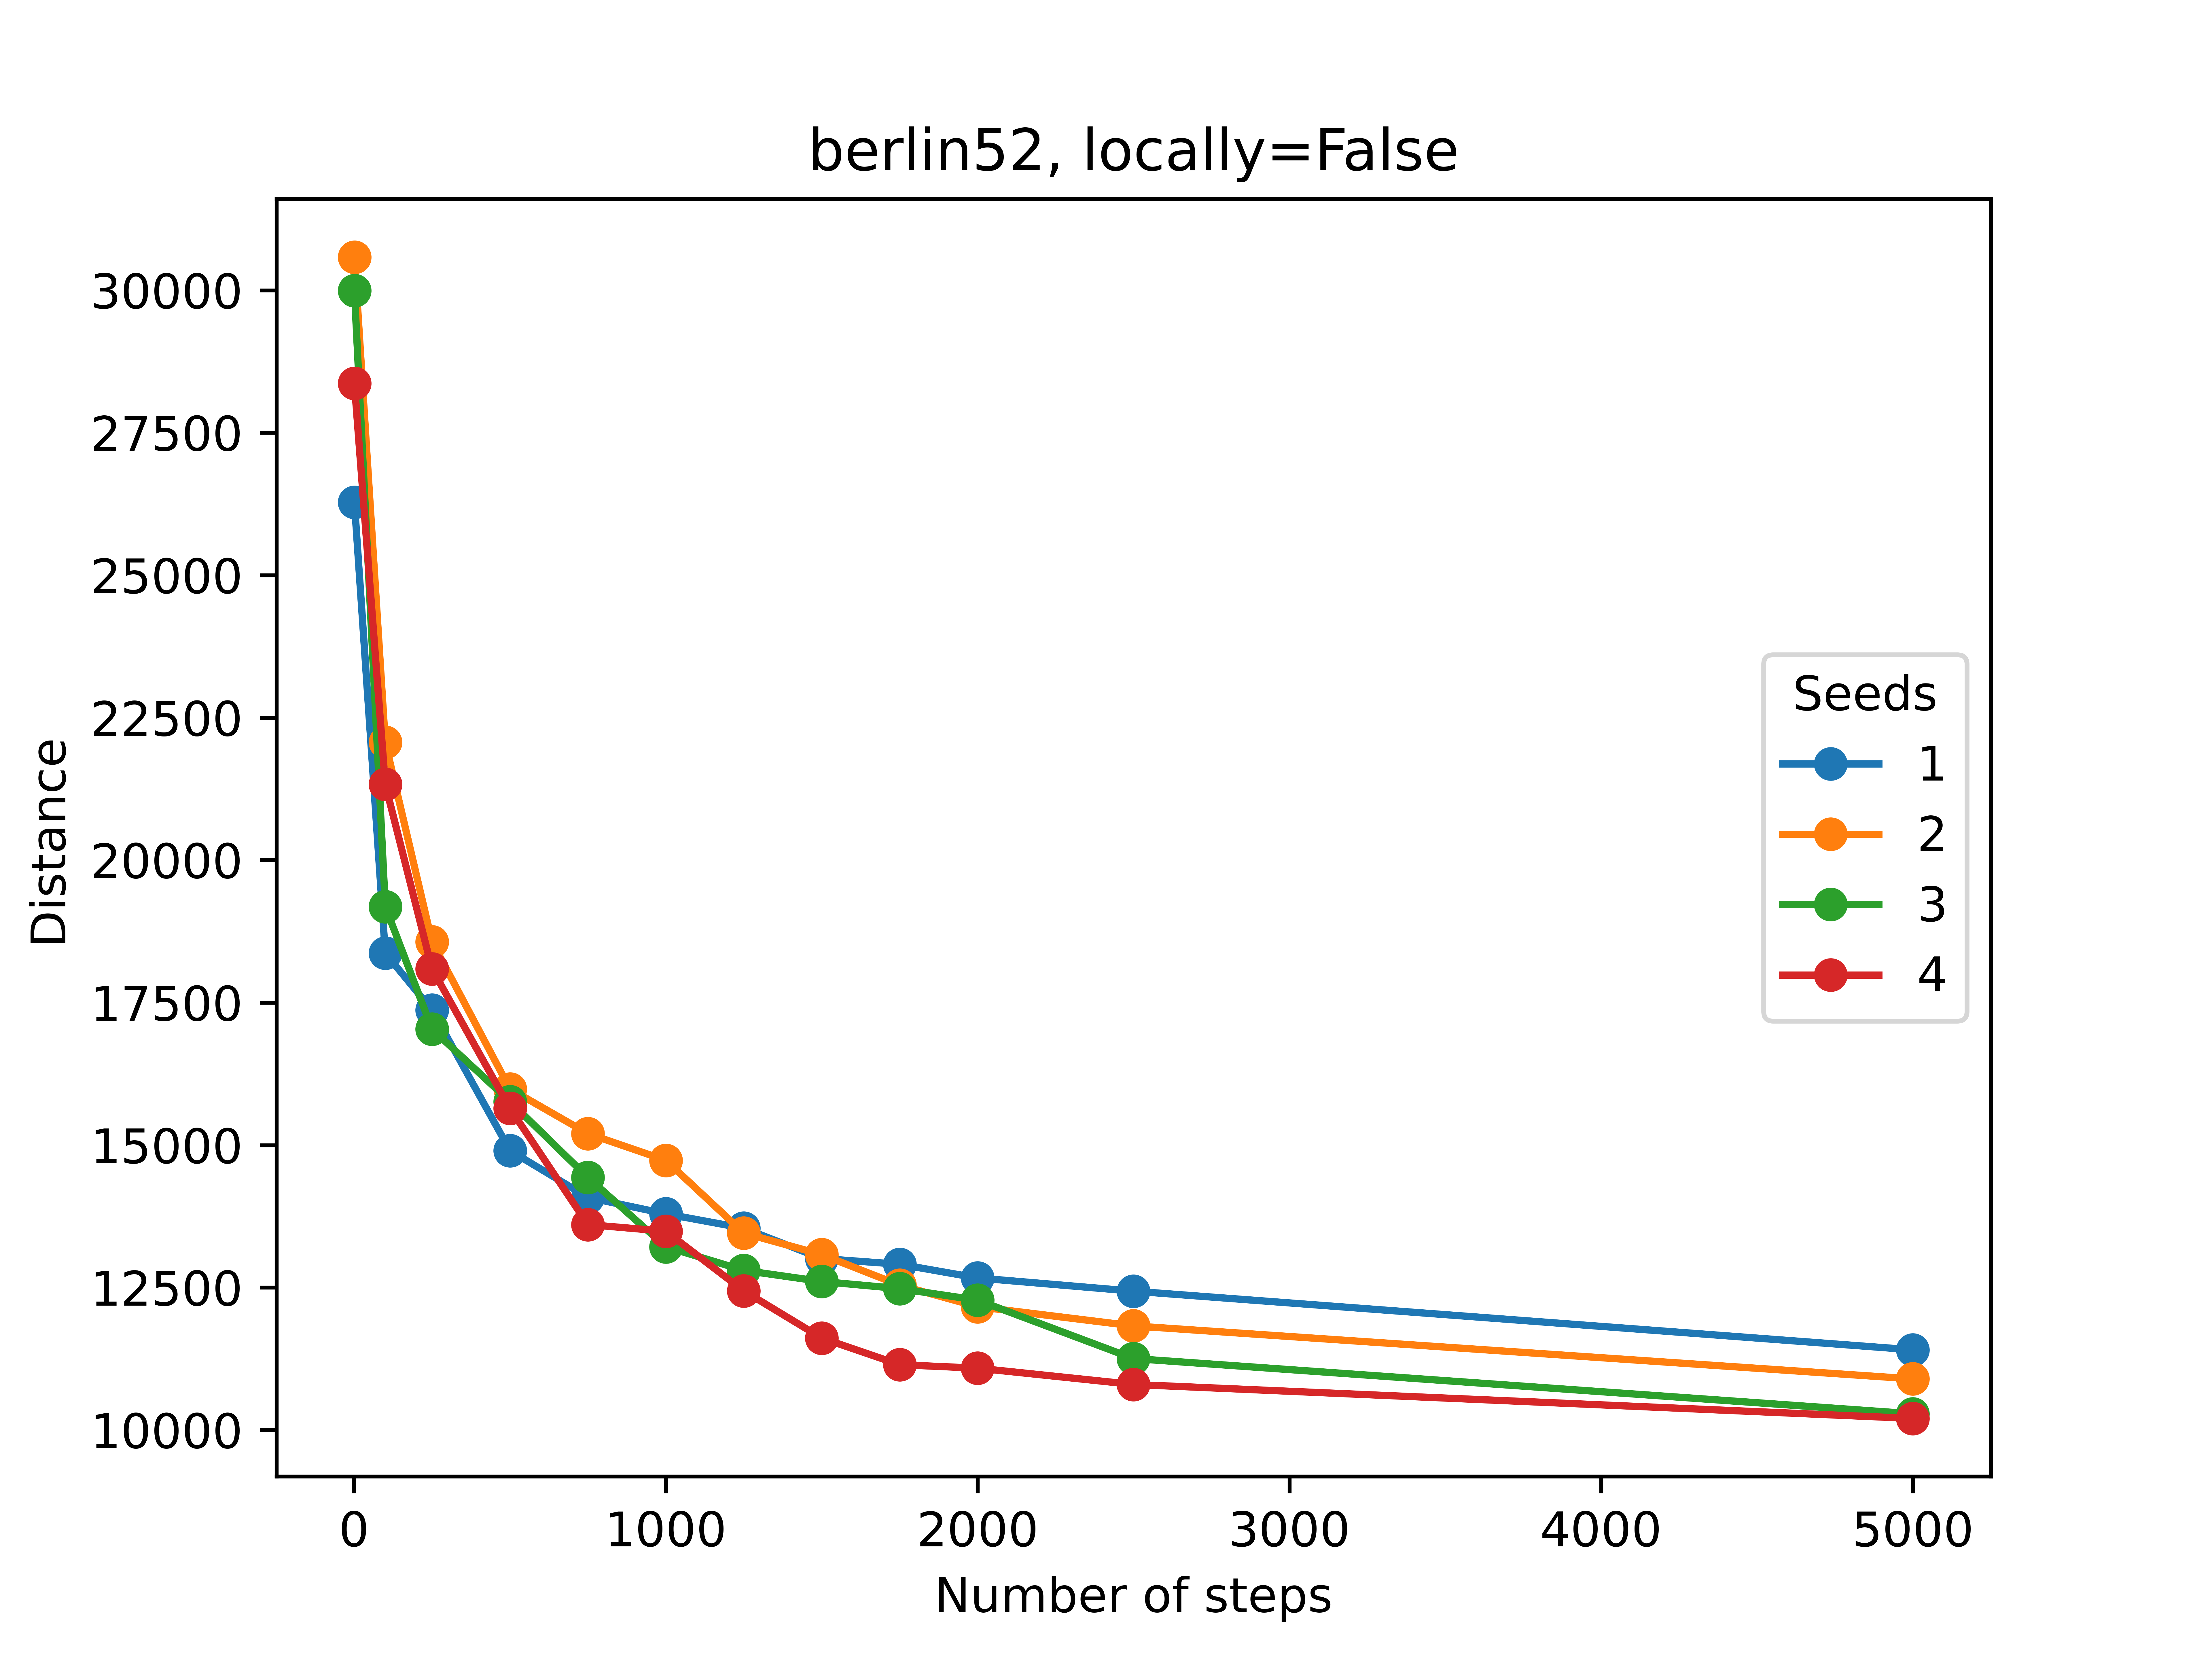
\includegraphics[width=\textwidth]{img/berlin52_seeds_locally=False}
		\subcaption{Random neighbours.}
	\end{subfigure}
	\begin{subfigure}{0.45\textwidth}
		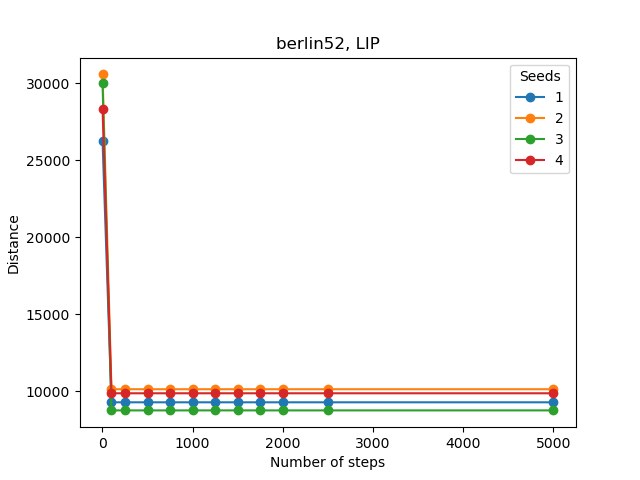
\includegraphics[width=\textwidth]{img/berlin52_seeds_locally=True}
		\subcaption{Locally-informed proposals.}
	\end{subfigure}
	\caption{Different initial states for \textit{berlin52}.}
	\label{fig:berlin52_seeds}
\end{figure}
	
\begin{figure}[!htb]
	\centering
	\begin{subfigure}{0.45\textwidth}
		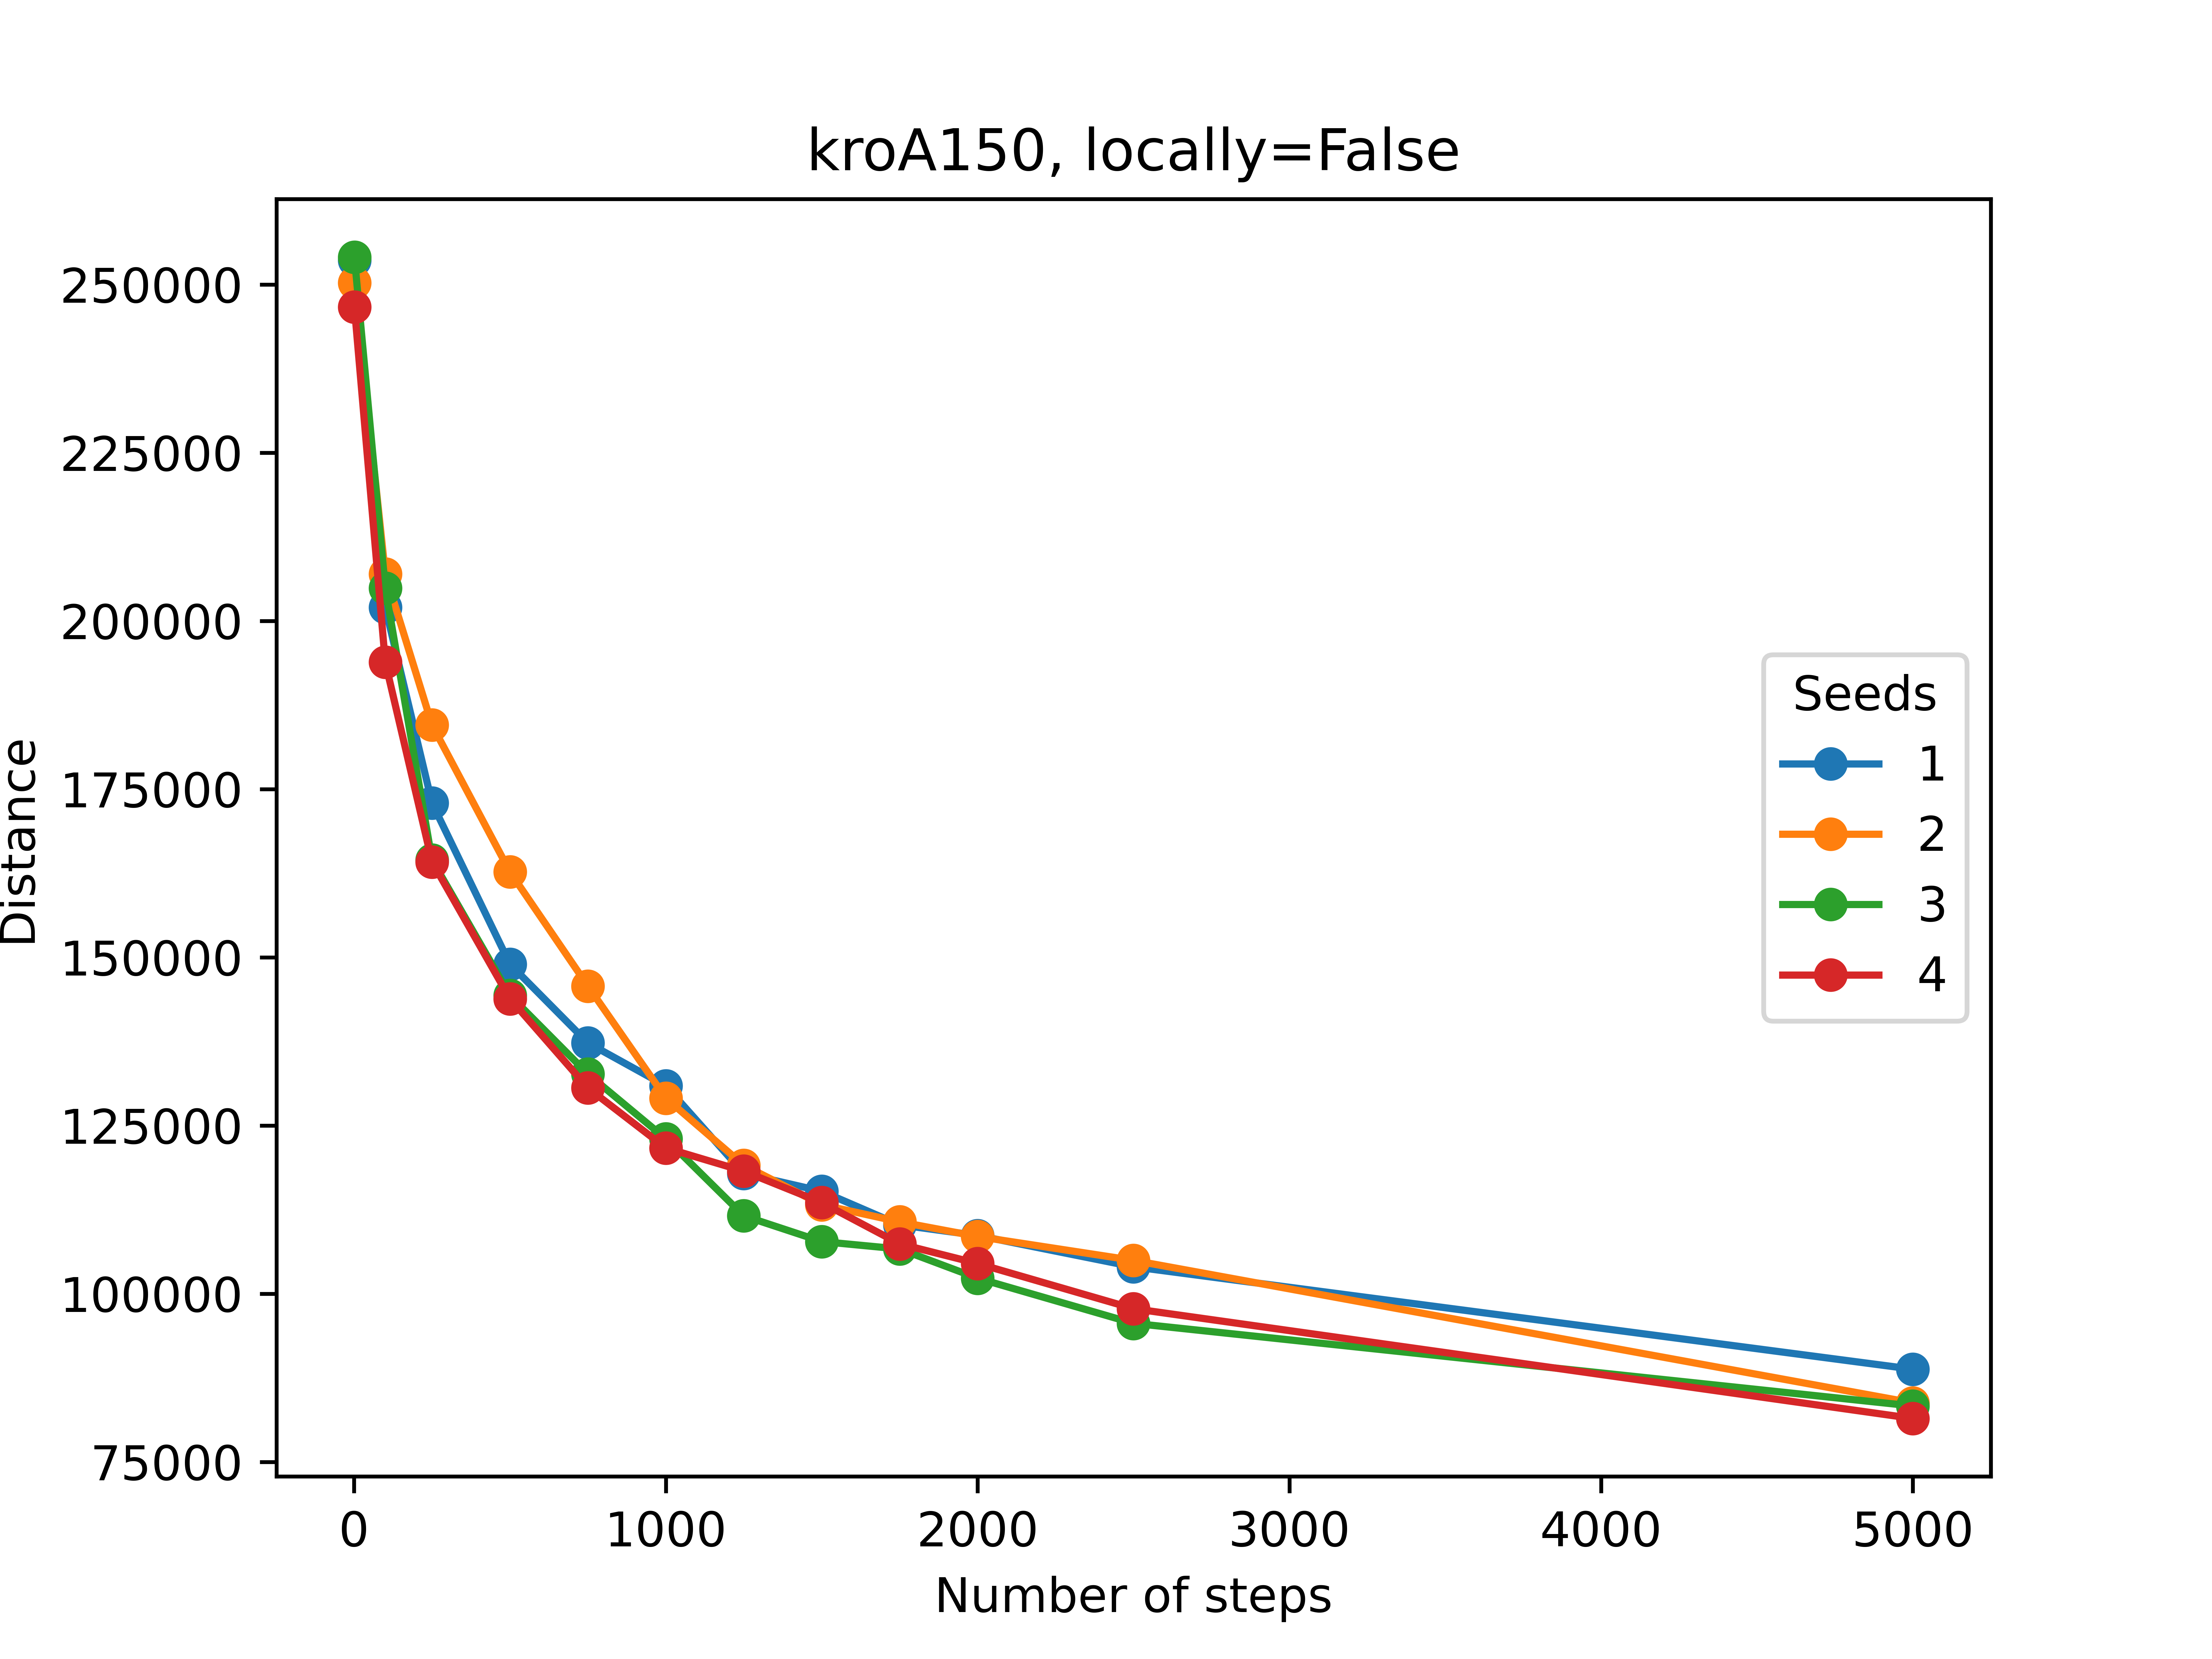
\includegraphics[width=\textwidth]{img/kroA150_seeds_locally=False}
		\subcaption{Random neighbours.}
	\end{subfigure}
	\begin{subfigure}{0.45\textwidth}
		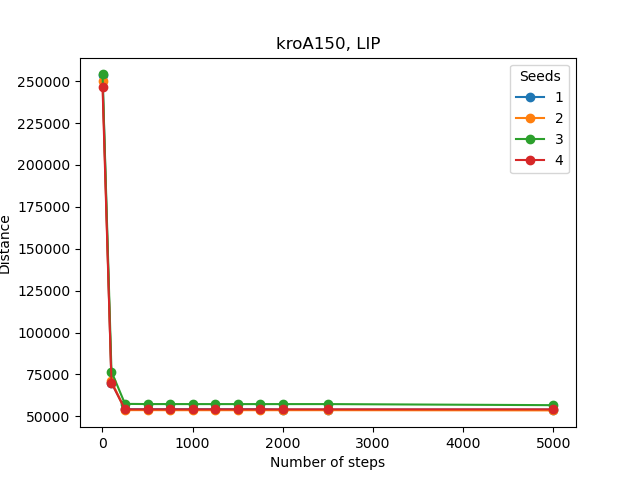
\includegraphics[width=\textwidth]{img/kroA150_seeds_locally=True}
		\subcaption{Locally-informed proposals.}
	\end{subfigure}
	\caption{Different initial states for \textit{kroA150}.}
	\label{fig:kroA150_seeds}
\end{figure}

	Both plots \ref{fig:berlin52_seeds} and \ref{fig:kroA150_seeds} suggest that initial state matters for finding a better tour, but it is not changing the behavior of algorithms.
	
\subsection{Simulated annealing}
	Before we proceed with comparing algorithms we need to find out if simulated annealing is improving them. We will compare parameters $t_n=1$ and $t_n= \frac{3}{\log(n+2)}$ where $n$ is a number of step. The temperature parameter for locally-informed proposals will stay at default $\tau=2$ and seed $1$.
	
	\begin{figure}[!htb]
	\centering
	\begin{subfigure}{0.45\textwidth}
		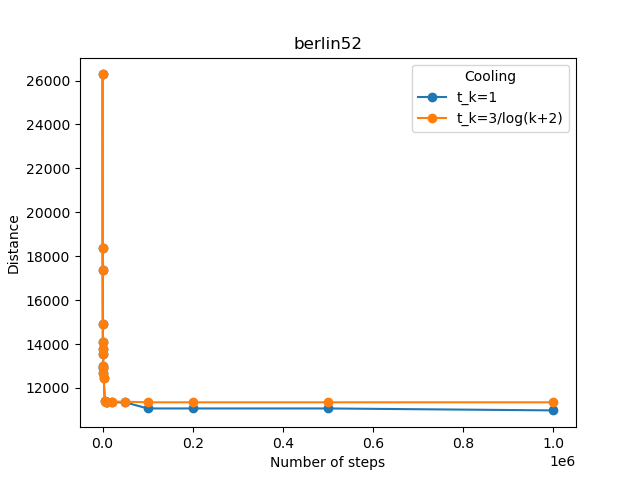
\includegraphics[width=\textwidth]{img/berlin52_annealing_locally=False}
		\subcaption{berlin52.}
	\end{subfigure}
	\begin{subfigure}{0.45\textwidth}
		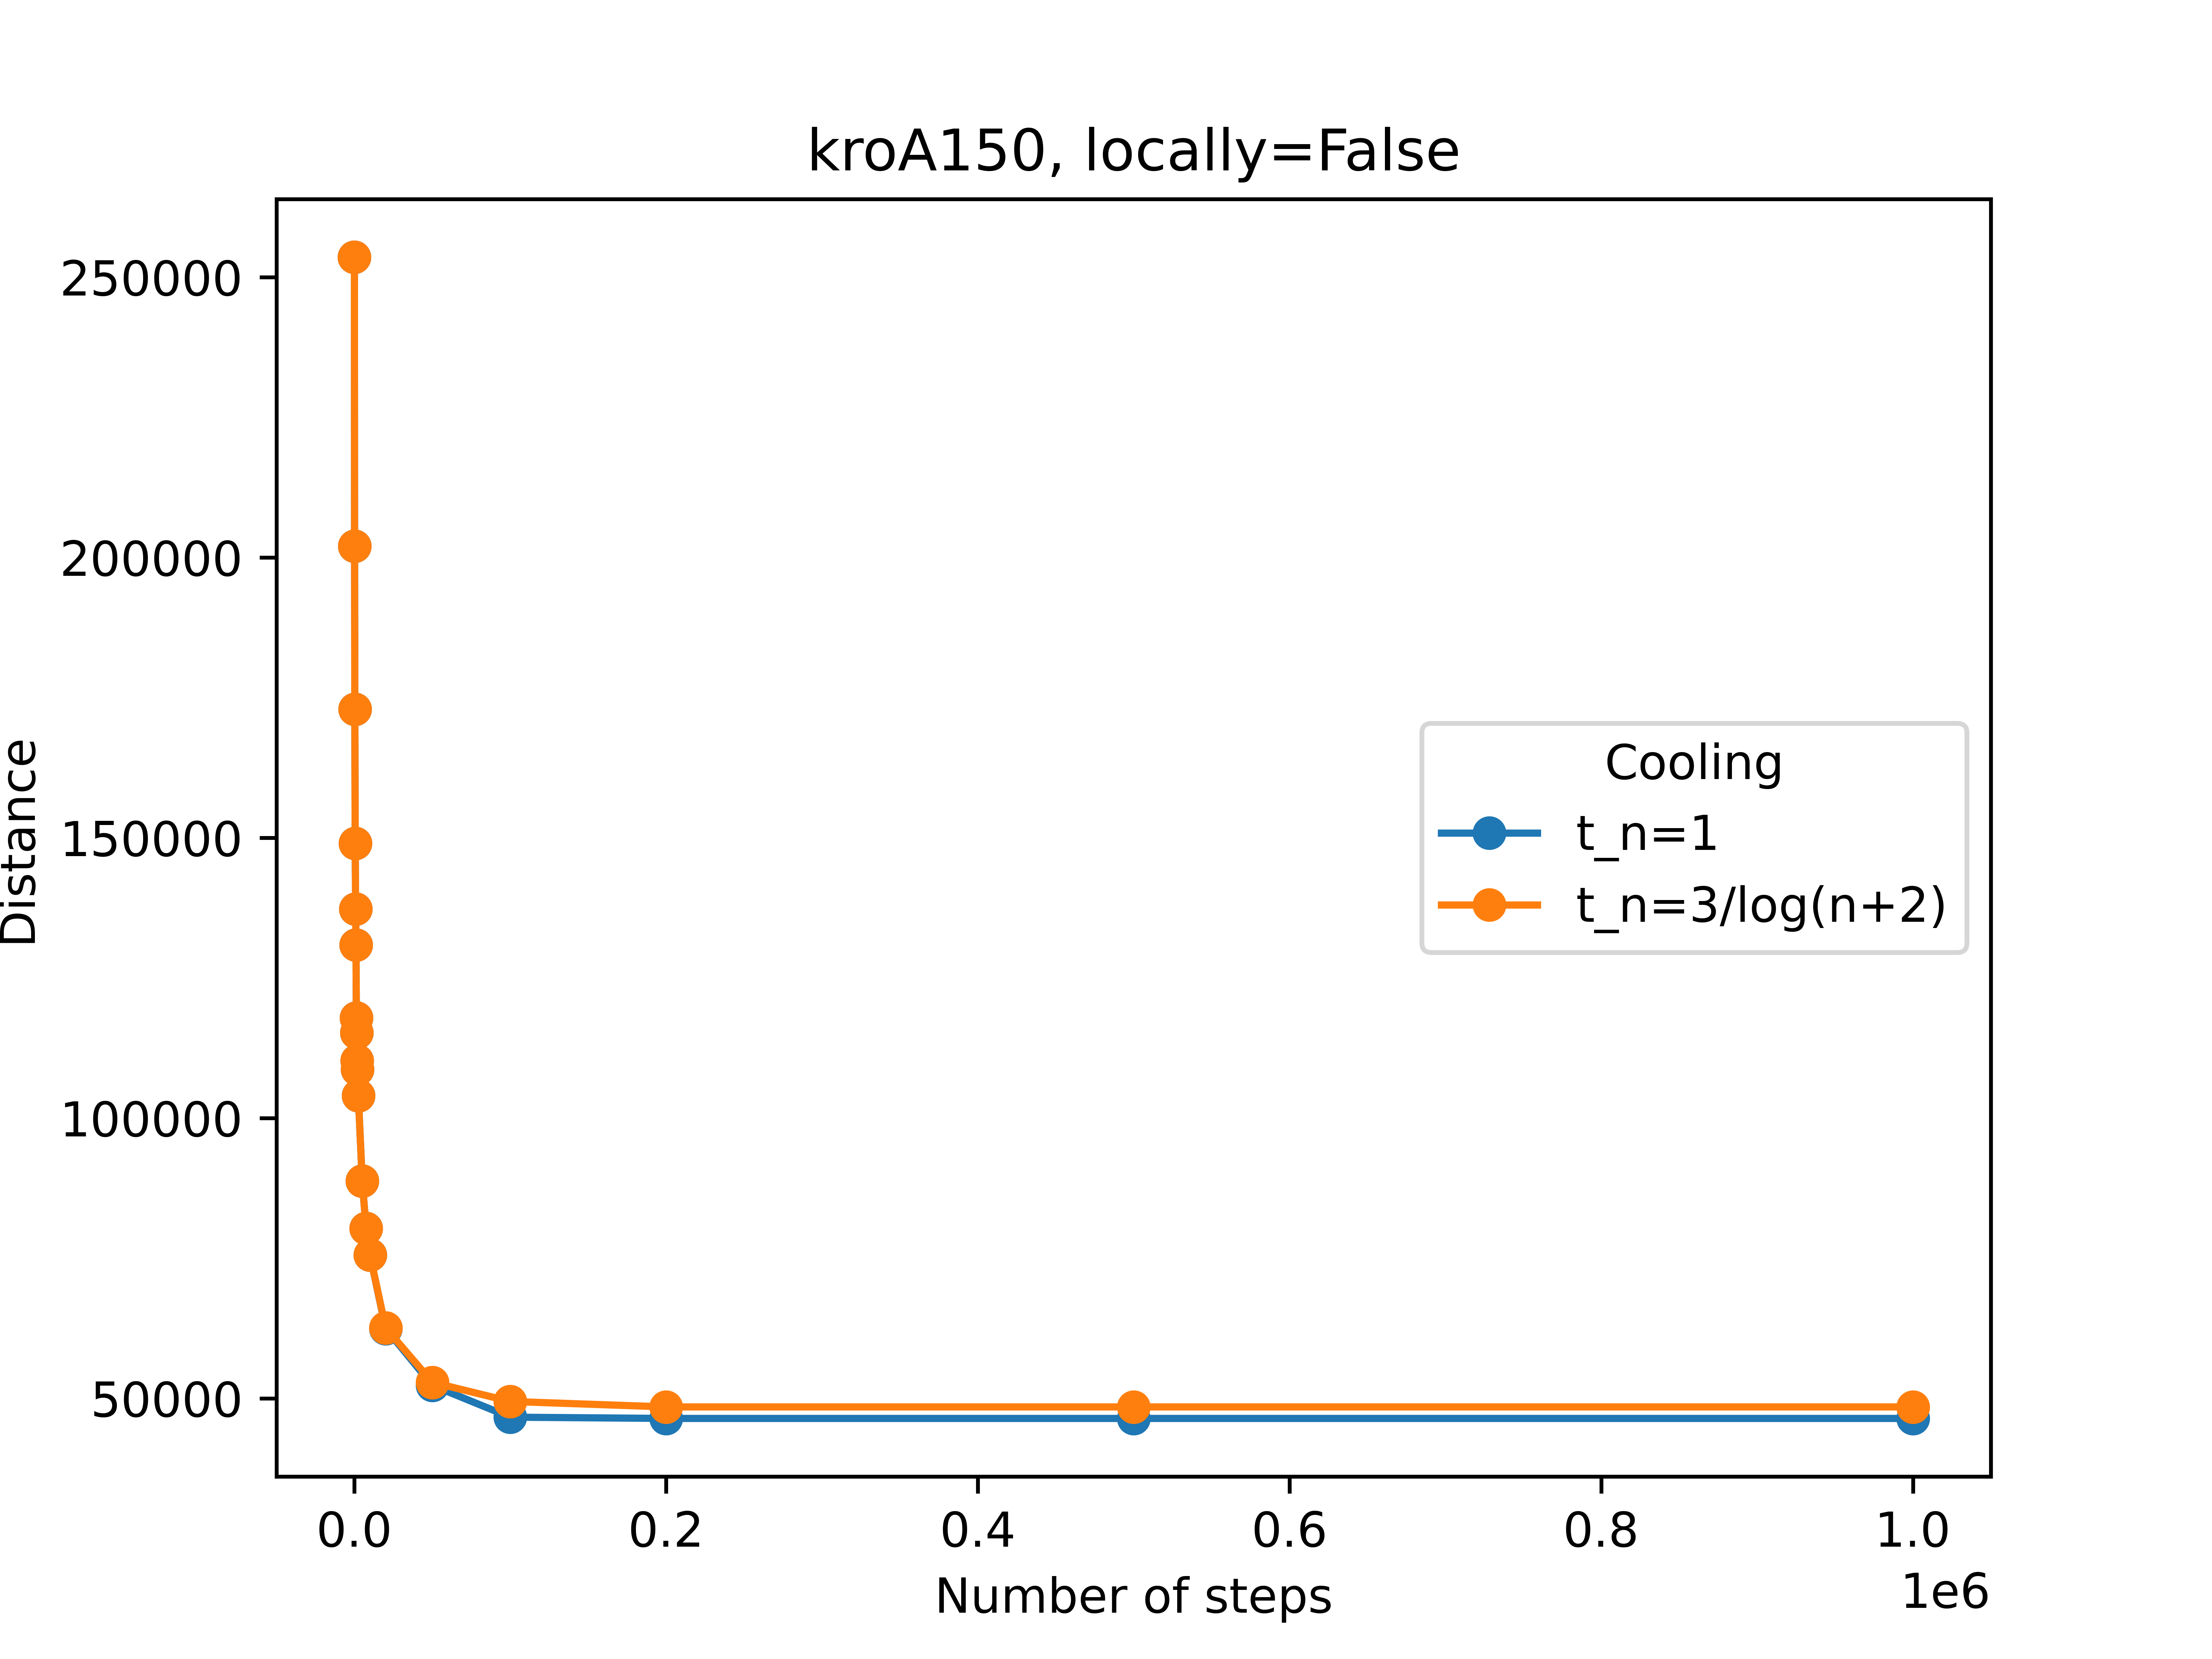
\includegraphics[width=\textwidth]{img/kroA150_annealing_locally=False}
		\subcaption{kroA150.}
	\end{subfigure}
	\caption{Distances over number of steps for 2 datasets with different cooling schedule.}
	\label{fig:annealing}
\end{figure}

	
	This time to see the difference between cooling parameters we had to extend number of iterations to 1 million. This number of steps is not viable for locally-informed proposals, so only random candidates were used. We can see slight the improvement at the end of iterations, which has potential when the distances are huge. 
	
\subsection{Temperature}
	The same needs to be done with temperature parameter $\tau$. It was proven in \cite{zanella2020informed} that $\tau=2$ is optimal for balancing out likelihoods, but maybe for this problem it is worth considering increasing some probability by this parameter.
	
	\begin{figure}[!htb]
	\centering
	\begin{subfigure}{0.45\textwidth}
		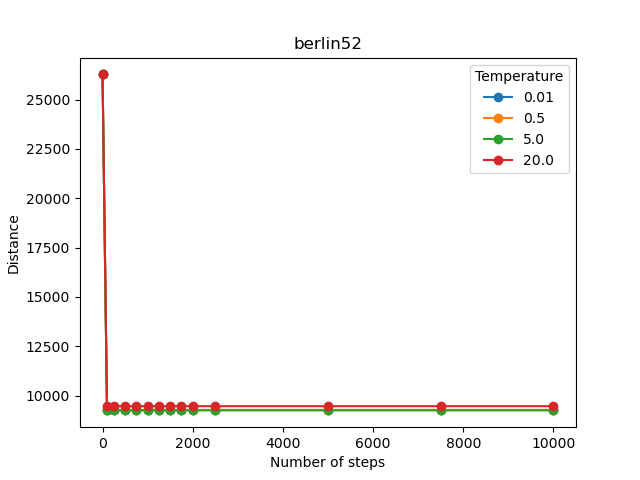
\includegraphics[width=\textwidth]{img/berlin52_temperature}
		\subcaption{berlin52.}
	\end{subfigure}
	\begin{subfigure}{0.45\textwidth}
		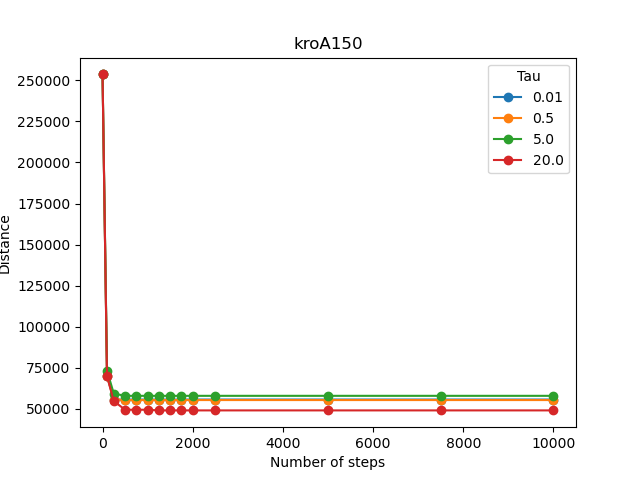
\includegraphics[width=\textwidth]{img/kroA150_temperature}
		\subcaption{kroA150.}
	\end{subfigure}
	\caption{Different temperature parameters for \textit{berlin52} and \textit{kroA150}.}
\end{figure}
	
	The plots \ref{fig:temperature_1} and \ref{fig:temperature_2} present LIP algorithm with the same initial state and different temperature parameter $\tau=0.01, 0.5, 5, 20$. For two datasets the results are almost identical, while on two others some temperatures offer better results, but they are not consistent with each other. This is why we opted for using $\tau=2$.
	
\subsection{Algorithms comparison}
	Now we are able to present all the results, we will be using $\tau=2$, two different cooling schedules $t_n=1, \, t_n=\frac{3}{\log(n+2)}$ and two different methods: random candidates and locally-informed proposals and the number of iterations is $5000$.
	
	\begin{figure}[!htb]
	\centering
	\begin{subfigure}{0.45\textwidth}
		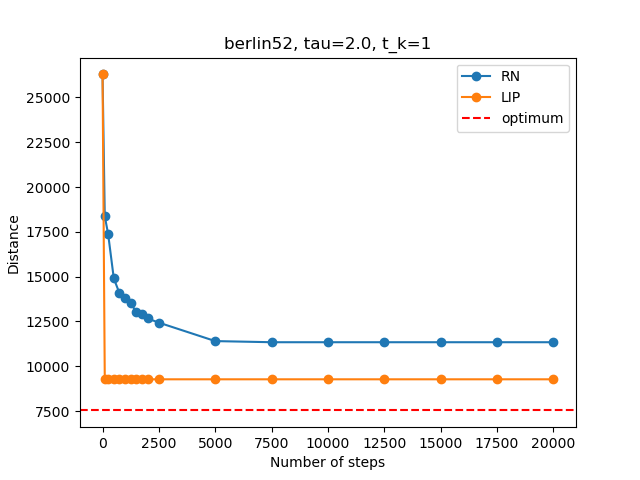
\includegraphics[width=\textwidth]{img/berlin52_temp=2.0_cool=1.0}
		\subcaption{$t_k=1$.}
	\end{subfigure}
	\begin{subfigure}{0.45\textwidth}
		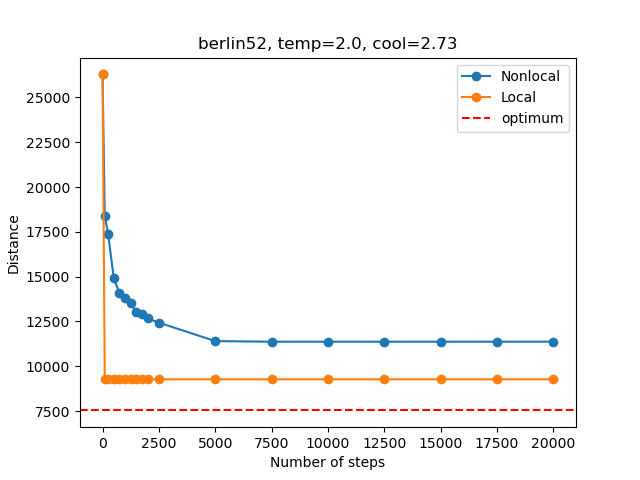
\includegraphics[width=\textwidth]{img/berlin52_temp=2.0_cool=2.73}
		\subcaption{$t_k=\frac{3}{\log(k+2)}$.}
	\end{subfigure}
	\caption{Comparing RN and LIP for \textit{berlin52} with different cooling parameters.}
	\label{fig:berlin52_comp}
\end{figure}
	
\begin{figure}[!htb]
	\centering
	\begin{subfigure}{0.45\textwidth}
		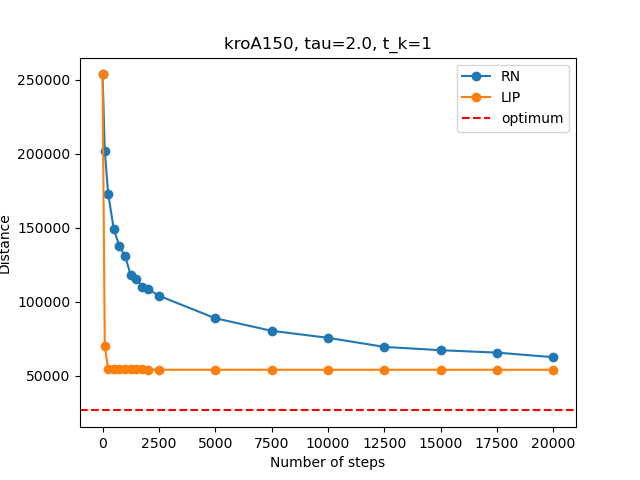
\includegraphics[width=\textwidth]{img/kroA150_temp=2.0_cool=1.0}
		\subcaption{$t_k=1$.}
	\end{subfigure}
	\begin{subfigure}{0.45\textwidth}
		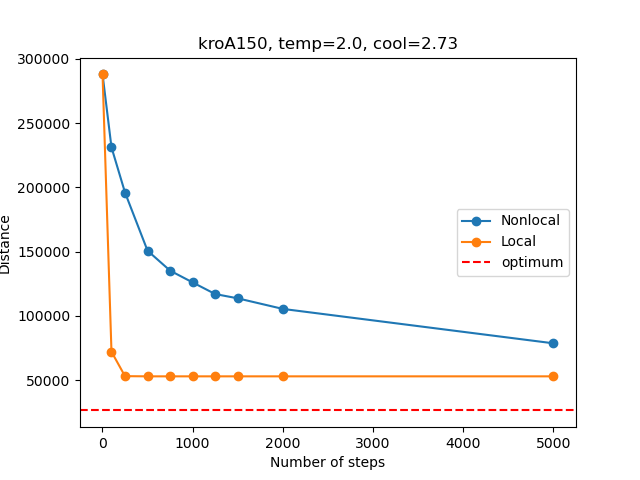
\includegraphics[width=\textwidth]{img/kroA150_temp=2.0_cool=2.73}
		\subcaption{$t_k=\frac{3}{\log(k+2)}$.}
	\end{subfigure}
	\caption{Comparing RN and LIP for \textit{kroA150} with different cooling parameters.}
	\label{fig:kroA150_comp}
\end{figure}

\begin{figure}[!htb]
	\centering
	\begin{subfigure}{0.45\textwidth}
		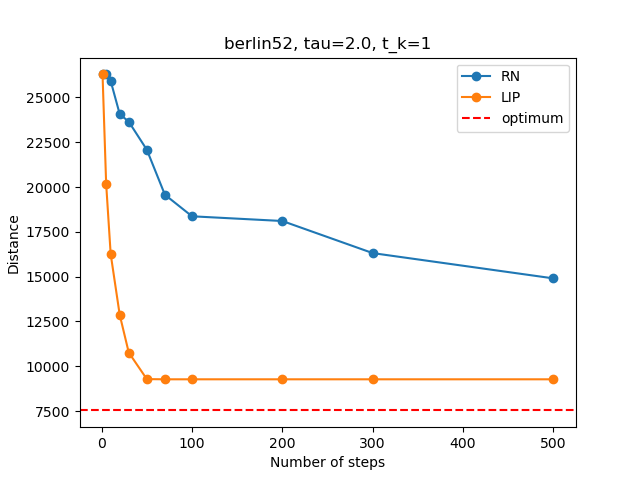
\includegraphics[width=\textwidth]{img/berlin52_temp=2.0_cool=1.0_low_iter}
		\subcaption{berlin52, $t_k=1$.}
	\end{subfigure}
	\begin{subfigure}{0.45\textwidth}
		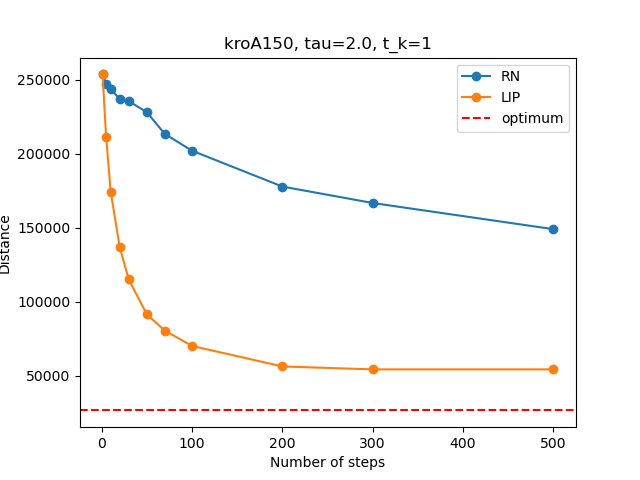
\includegraphics[width=\textwidth]{img/kroA150_temp=2.0_cool=1.0_low_iter}
		\subcaption{kroA150, $t_k=1$.}
	\end{subfigure}
	\caption{Comparing RN and LIP for \textit{berlin52} and \textit{kroA150} with low number of iterations.}
	\label{fig:low_iter}
\end{figure}

\begin{figure}[!htb]
	\centering
	\begin{subfigure}{0.45\textwidth}
		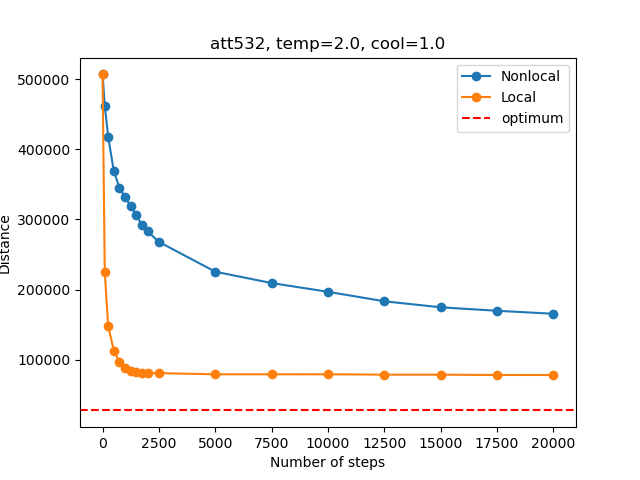
\includegraphics[width=\textwidth]{img/att532_temp=2.0_cool=1.0}
		\subcaption{$t_k=1$.}
	\end{subfigure}
	\begin{subfigure}{0.45\textwidth}
		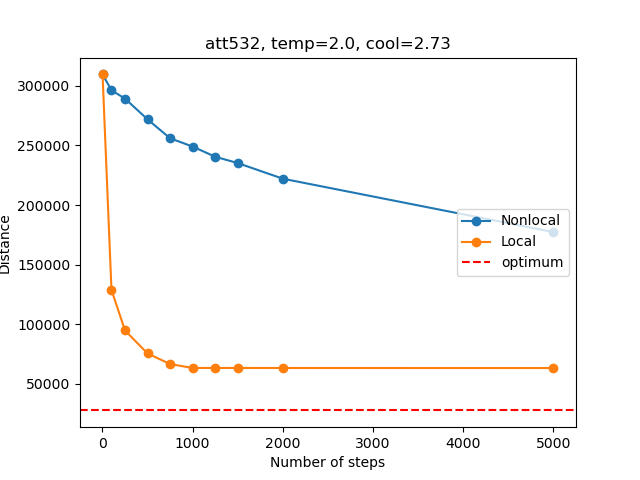
\includegraphics[width=\textwidth]{img/att532_temp=2.0_cool=2.73}
		\subcaption{$t_k=\frac{3}{\log(k+2)}$.}
	\end{subfigure}
	\caption{Comparing RN and LIP for \textit{att532} with different cooling parameters.}
	\label{fig:att532_comp}
\end{figure}

\begin{figure}[!htb]
	\centering
	\begin{subfigure}{0.45\textwidth}
		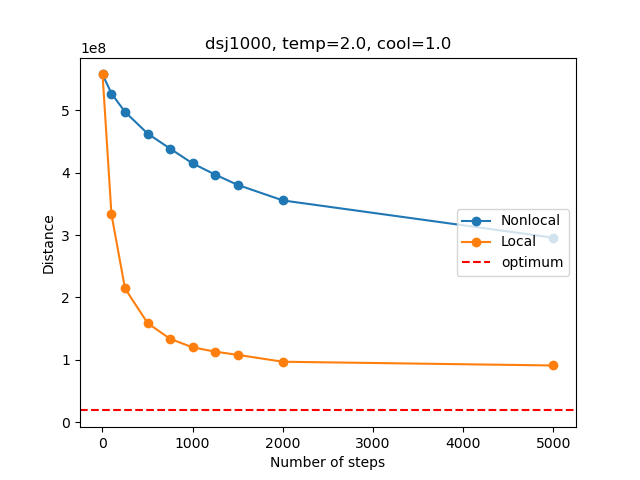
\includegraphics[width=\textwidth]{img/dsj1000_temp=2.0_cool=1.0}
		\subcaption{$t_k=1$.}
	\end{subfigure}
	\begin{subfigure}{0.45\textwidth}
		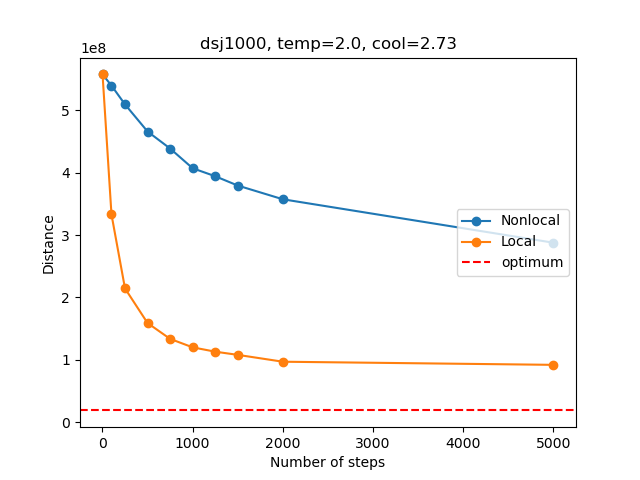
\includegraphics[width=\textwidth]{img/dsj1000_temp=2.0_cool=2.73}
		\subcaption{$t_k=\frac{3}{\log(k+2)}$.}
	\end{subfigure}
	\caption{Comparing RN and LIP for \textit{dsj1000} with different cooling parameters.}
	\label{fig:dsj1000_comp}
\end{figure}
	
	The plots \ref{fig:berlin52_comp}, \ref{fig:kroA150_comp}, \ref{fig:att532_comp}, \ref{fig:dsj1000_comp} present distance of a solution as a function of number of steps. Both algorithms start at the same state and have the same seed. We can se how quickly they diverge. First steps of locally-informed proposals algorithm is taking the best neighbours it can and stays there or makes small improvements. Prolonged stays happen in smaller datasets as there is less deviation at each step and it is harder to choose a better neighbour. At the beginning LIP algorithm has obviously better results in all cases.
	
	Additionally the plot \ref{fig:low_iter} compares two methods but on a shorter distances and only for two smaller dataset. The number of vertices is smaller, so LIP finds better solutions quickly and it is easier to compare the methods with fewer iterations. We can see, that less than 100 iterations are enough to create a massive gap between these methods.
	
	\begin{table}[!htb]
	\centering
	\footnotesize
	\begin{tabular}{l|lll|lll|}
		\cline{2-7}
		& \multicolumn{3}{l|}{RN}                                        & \multicolumn{3}{l|}{LIP}                                          \\ \hline
		\multicolumn{1}{|l|}{dataset}  & \multicolumn{1}{l|}{dist.}     & \multicolumn{1}{l|}{time $[s]$} & ratio & \multicolumn{1}{l|}{dist.}    & \multicolumn{1}{l|}{time $[s]$} & ratio \\ \hline
		\multicolumn{1}{|l|}{berlin52} & \multicolumn{1}{l|}{11344}     & \multicolumn{1}{l|}{1.32} & 1.50  & \multicolumn{1}{l|}{9276}     & \multicolumn{1}{l|}{116}  & 1.23  \\ \hline
		\multicolumn{1}{|l|}{kroA150}  & \multicolumn{1}{l|}{62467}     & \multicolumn{1}{l|}{1.24} & 2.36  & \multicolumn{1}{l|}{53988}    & \multicolumn{1}{l|}{454}  & 2.04  \\ \hline
		\multicolumn{1}{|l|}{att532}   & \multicolumn{1}{l|}{165445}    & \multicolumn{1}{l|}{1.38} & 5.98  & \multicolumn{1}{l|}{78150}    & \multicolumn{1}{l|}{2462} & 2.82  \\ \hline
		\multicolumn{1}{|l|}{dsj1000}  & \multicolumn{1}{l|}{199343433} & \multicolumn{1}{l|}{1.5}  & 10.68 & \multicolumn{1}{l|}{89105687} & \multicolumn{1}{l|}{6439} & 4.78  \\ \hline
	\end{tabular}
	\caption{Methods comparison, $t_k=1$, 20000-th step.}
\end{table}
	
	The tables \ref{tab:results_comp_cool=1} and \ref{tab:results_comp_cool=2.73} present comparison of those two methods for different cooling parameters. They contain distances of tours, time the algorithm took and ratio of the solution to the optimum. For bigger datasets the ratio is growing, which is behaving as expected -- the more vertices to search through, so more iterations are needed to reach optimum. The LIP algorithm outperforms random candidates, given small amount of iterations. We can also notice that the cooling parameter does not cause any significant difference.